\section{Experimento 3: Modelos con mayor complejidad}
\label{sec:combinacion_variables}

\subsection{Selección del subconjunto de variables}

Los Experimentos 1 y 2 (Secciones \ref{sec:resultados_features_original} y \ref{sec:resultados_features_transformadas}) evaluaron
la contribución individual de cada variable al modelo base MD2, considerando tanto su escala
original como sus versiones transformadas cuando correspondía. Para construir un modelo
combinado de mayor complejidad es necesario reducir el conjunto de 15
variables candidatas a un subconjunto que combine capacidad predictiva individual demostrada
con baja redundancia entre sí. Este proceso de selección se realizó en tres pasos:

\paragraph{Paso 1: Selección de versión (original vs. transformada).}
\begin{sloppypar}
Para las variables en las que se exploró una transformación logarítmica, se priorizó la
versión que presentó un cluster espacio-temporal significativo según TFCE, y en los casos
en que ambas versiones resultaron significativas el desempate se realizó según el
$\Delta$AIC obtenido. De este proceso resultaron seleccionadas las versiones
\feat{saliencia\_media}, \feat{saliencia\_pixel\_log},
\feat{similitud\_media\_log}, \feat{similitud\_pixel\_log},
\feat{evidencia\_visual}, \feat{competencia\_fp\_var},
\feat{competencia\_fp\_media}, \feat{competencia\_fp\_max\_log},
\feat{posterior}, \feat{entropia\_prior\_saliencia}, \feat{entropia\_posterior},
\feat{ganancia\_informacion\_log}, \feat{gap\_entropia\_log},
\feat{distancia\_grilla} y \feat{competencia\_densidad}. De estas 15 variables,
5 corresponden a su versión transformada (\feat{saliencia\_pixel\_log},
\feat{similitud\_media\_log}, \feat{similitud\_pixel\_log},
\feat{competencia\_fp\_max\_log} y \feat{gap\_entropia\_log}), mientras que las
10 restantes se mantienen en su escala original, ya sea porque no se exploró
ninguna transformación para ellas o porque la versión transformada fue
descartada previamente por VIF o por no aportar mejoras.
\end{sloppypar}

\paragraph{Paso 2: Filtro por significancia estadística.}
Del conjunto de 15 variables evaluadas en el Paso 1, se conservaron únicamente aquellas
que presentaron al menos una versión (original o transformada) con cluster
espacio-temporal significativo según TFCE. Este criterio redujo el conjunto a 7 variables:
\feat{saliencia\_pixel\_log}, \feat{saliencia\_media}, \feat{similitud\_pixel\_log},
\feat{similitud\_media\_log}, \feat{posterior}, \feat{ganancia\_informacion\_log}
y \feat{gap\_entropia\_log}.

\paragraph{Paso 3: Reducción por redundancia intra-categoría.}
Cuando más de una variable de las 7 anteriores pertenecía a la misma categoría conceptual
(bottom-up, similitud con el target), se conservó únicamente la de mayor $\Delta$AIC
individual, descartando el resto por redundancia. Este criterio redujo el conjunto a
5 variables: \feat{saliencia\_pixel\_log}, \feat{similitud\_pixel\_log},
\feat{posterior}, \feat{ganancia\_informacion\_log} y \feat{gap\_entropia\_log}.

\subsection{Multicolinealidad por VIF}
\begin{sloppypar}
Se calculó el VIF de las 5 variables incorporándolas simultáneamente al modelo
base MD2, descartando aquellas con VIF elevado en la mayoría de los sujetos. Este criterio
redujo el conjunto al subconjunto final de 4 variables:
\feat{saliencia\_pixel\_log}, \feat{similitud\_pixel\_log}, \feat{posterior}
y \feat{gap\_entropia\_log}. La variable \feat{ganancia\_informacion\_log} superó el umbral
de VIF $>$ 5 en más de la mitad de los sujetos.
\end{sloppypar}

\begin{table}[H]
\centering
\small
\begin{tabular}{lcccc}
\toprule
\textbf{Variable} & \textbf{Media} & \textbf{Mediana} & \textbf{\% sujetos VIF $>$ 3} & \textbf{\% sujetos VIF $>$ 5} \\
\midrule
\multicolumn{5}{l}{\textit{Predictores del modelo base}} \\
ontarget                 & 2.18 & 2.19 & 0.0   & 0.0 \\
mss                      & 3.19 & 3.18 & 71.4  & 0.0 \\
correct                  & 2.80 & 2.70 & 31.0  & 2.4 \\
scrank                   & 1.19 & 1.19 & 0.0   & 0.0 \\
\midrule
\multicolumn{5}{l}{\textit{Variables candidatas al modelo combinado}} \\
saliencia\_pixel\_log         & 3.52 & 3.49 & 100.0 & 0.0 \\
similitud\_pixel\_log         & 3.46 & 3.44 & 100.0 & 0.0 \\
posterior                     & 1.55 & 1.53 & 0.0   & 0.0 \\
ganancia\_informacion\_log    & 5.07 & 5.07 & 100.0 & 54.8 \\
gap\_entropia\_log            & 1.85 & 1.84 & 0.0   & 0.0 \\
\bottomrule
\end{tabular}
\caption{VIF calculado por sujeto al incorporar simultáneamente las 5 variables
candidatas al modelo base MD2. Se reportan la media y mediana grupal ($n=42$) y el
porcentaje de sujetos que superan los umbrales de VIF $>$ 3 y VIF $>$ 5, tanto para
los predictores del modelo base como para las variables candidatas.
\feat{ganancia\_informacion\_log} fue la única variable candidata en superar el umbral
de VIF $>$ 5 en más de la mitad de los sujetos, por lo que fue excluida del modelo
combinado final.}
\label{tab:vif_combinado_5}
\end{table}

\subsection{Resultados}

Para evaluar la contribución conjunta de las 4 variables seleccionadas en la sección
anterior se construyeron tres variantes del Experimento 3,
incorporando de forma incremental los resultados de significancia obtenidos en cada
iteración.

\paragraph{Experimento 3a.} Se incorporaron simultáneamente al modelo base MD2 las
4 variables del subconjunto final: \feat{saliencia\_pixel\_log},
\feat{similitud\_pixel\_log}, \feat{posterior} y \feat{gap\_entropia\_log}.

\paragraph{Experimento 3b.} Dado que \feat{posterior} no presentó cluster
espacio-temporal significativo según TFCE en el Experimento 3a, se la excluyó del
modelo, quedando un modelo combinado de 3 variables: \feat{saliencia\_pixel\_log},
\feat{similitud\_pixel\_log} y \feat{gap\_entropia\_log}.

\paragraph{Experimento 3c.} Dado que \feat{similitud\_pixel\_log} tampoco presentó
cluster significativo en el Experimento 3b, se la excluyó también, quedando un
modelo combinado final de 2 variables: \feat{saliencia\_pixel\_log} y
\feat{gap\_entropia\_log}.

La Figura~\ref{fig:resultados_combinados} presenta los mapas espacio-temporales de significancia TFCE de todas las variables involucradas en cada uno de los experimentos.

\begin{figure}[H]
    \centering
    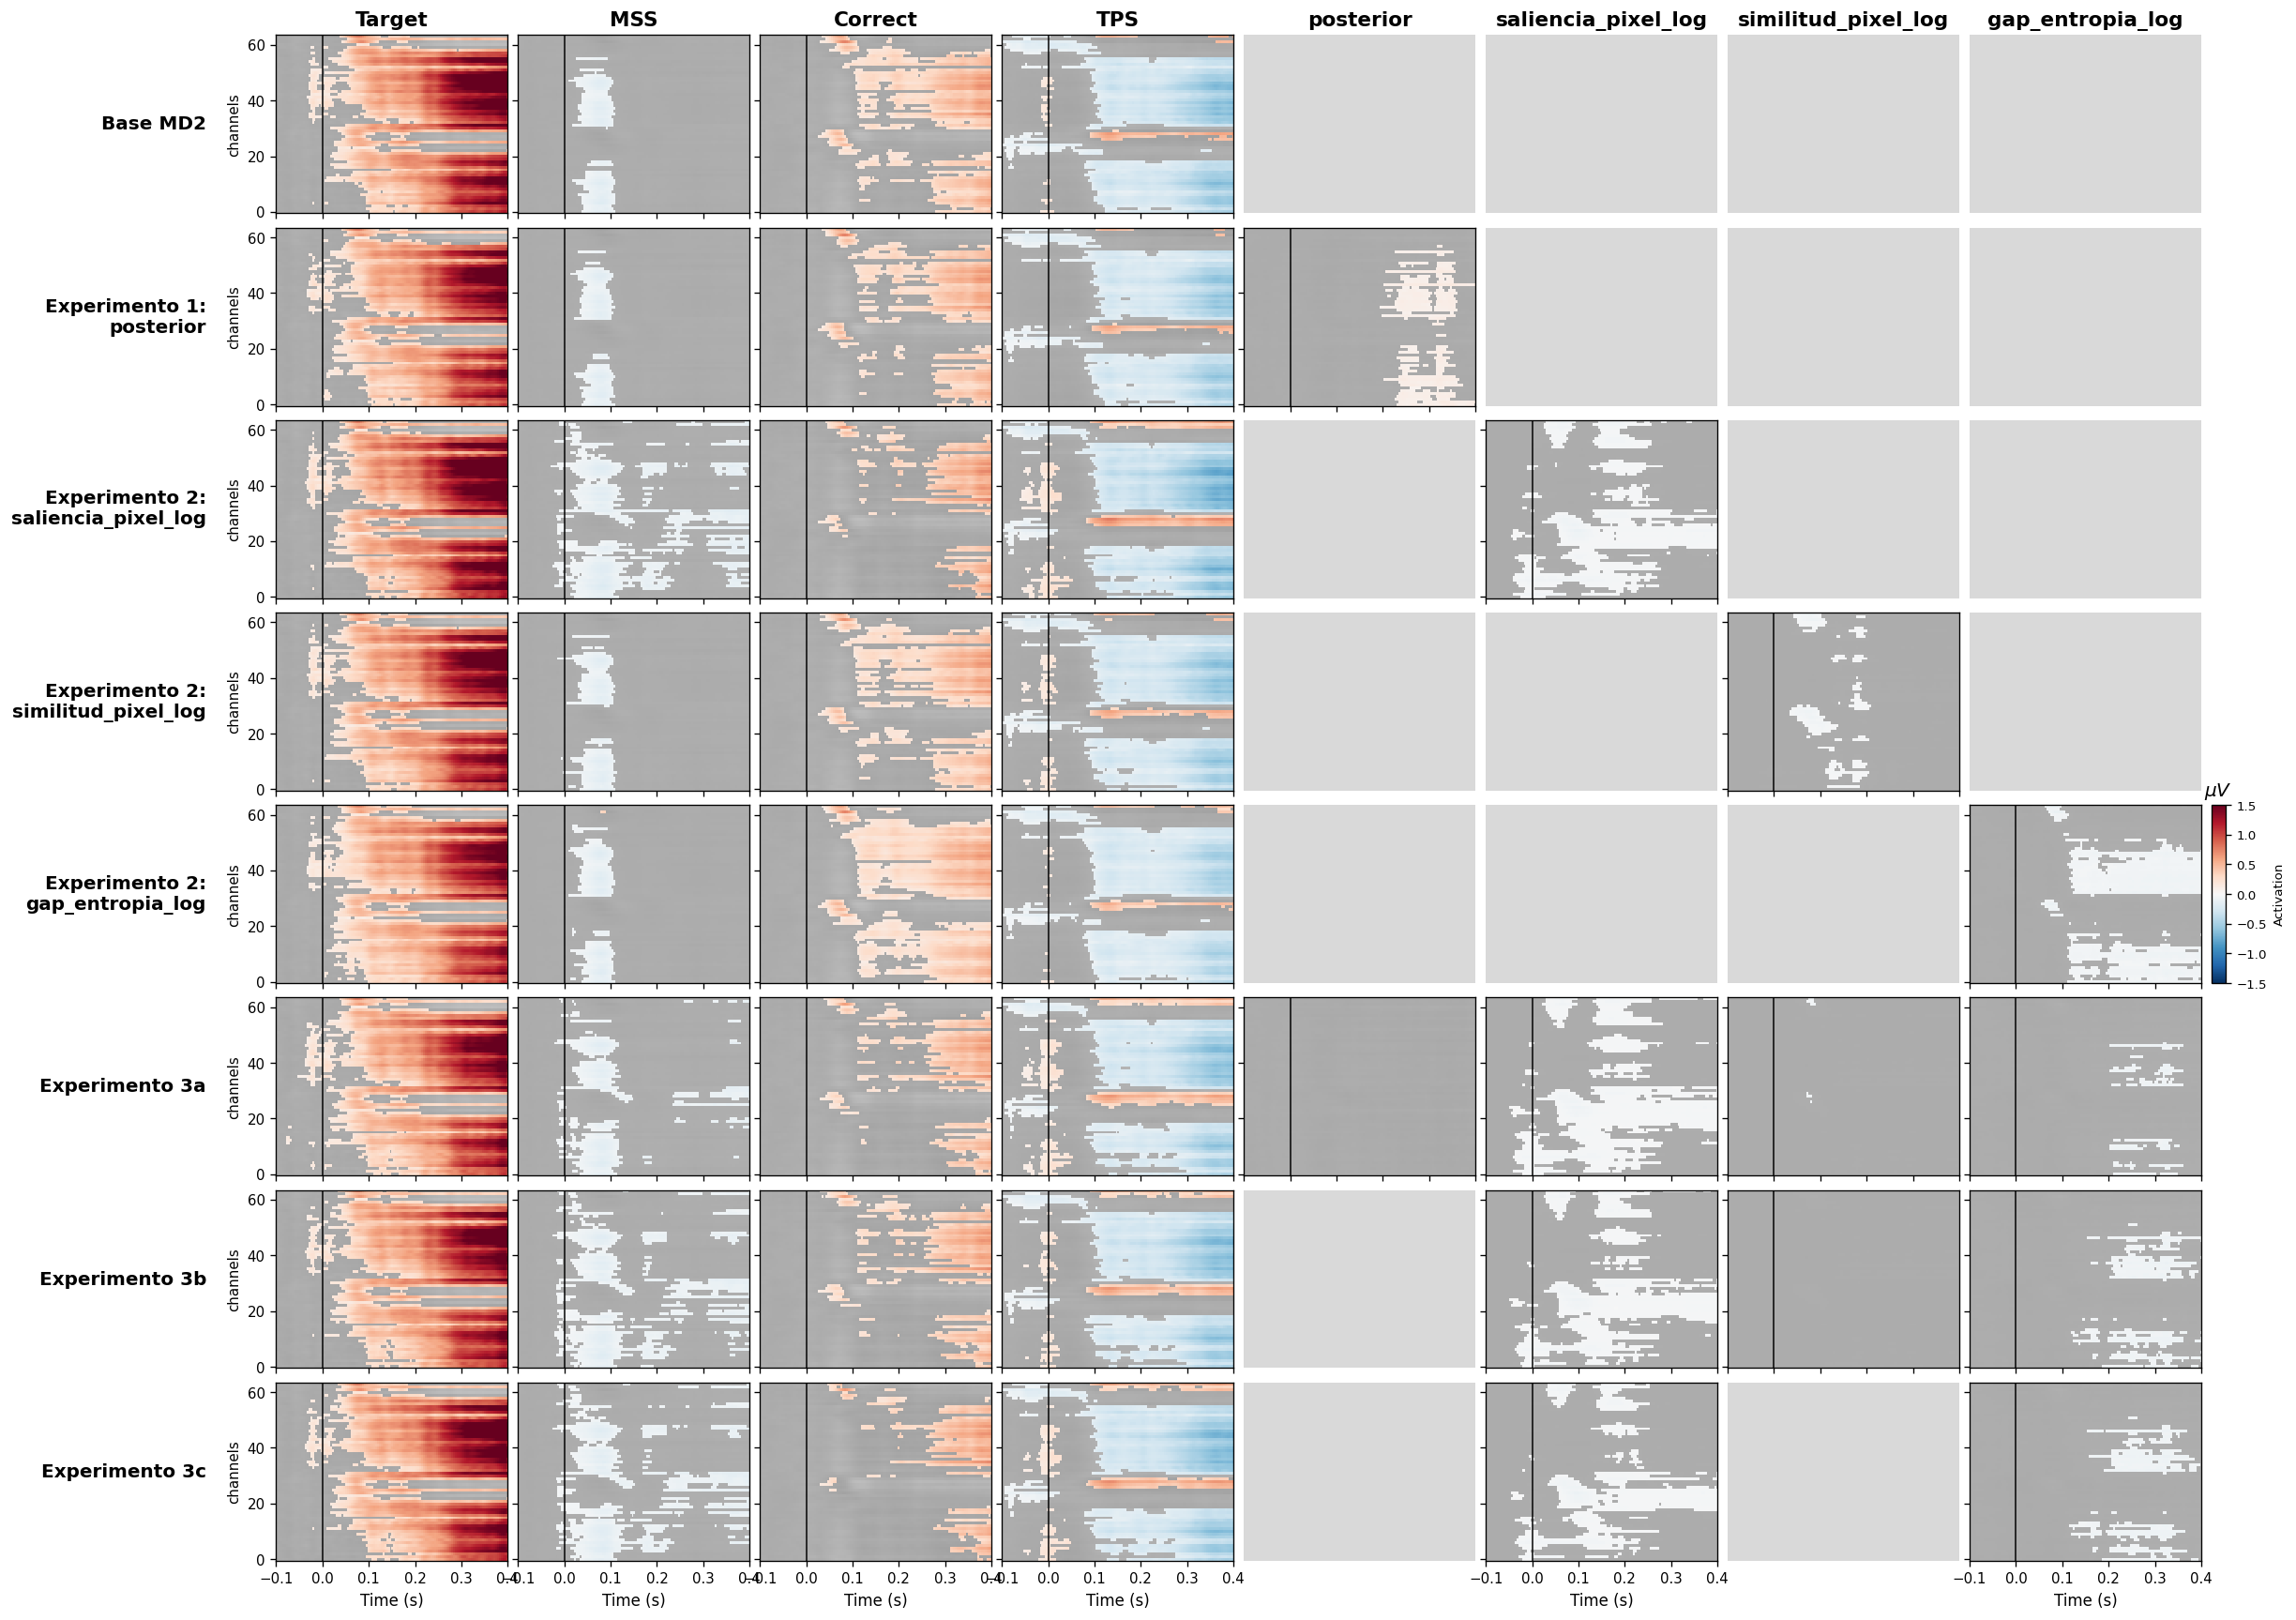
\includegraphics[width=\textwidth]{chapters/05_resultados/images/TFCE-final.png}
    \caption{Resultados TFCE para las variables con clusters significativos en escala original: \feat{posterior}, \feat{saliencia\_media}, \feat{saliencia\_pixel} y \feat{similitud\_pixel}.}
    \label{fig:resultados_combinados}
\end{figure}

%\begin{figure}[H]
%\centering
%\includegraphics[width=\textwidth]{figuras/resultados_combinados.png}
%\caption{Comparación de resultados TFCE entre el modelo base MD2, los %Experimentos 1
%y 2 (variables incorporadas individualmente) y los Experimentos 3a y 3b del %modelo
%combinado. Cada fila corresponde a una variante del modelo; cada columna, %a un
%predictor. Los paneles en blanco indican predictores no incluidos en esa %variante del
%modelo. \textit{Pendiente: agregar fila correspondiente al Experimento %3c.}}
%\label{fig:resultados_combinados}
%\end{figure}

La Figura~\ref{fig:aic_combinados} compara el $\Delta$AIC de los modelos combinados
(Experimentos 3a y 3b) contra el $\Delta$AIC obtenido por cada variable al incorporarse
individualmente al modelo base MD2 (Experimentos 1 y 2).

\begin{figure}[H]
\centering
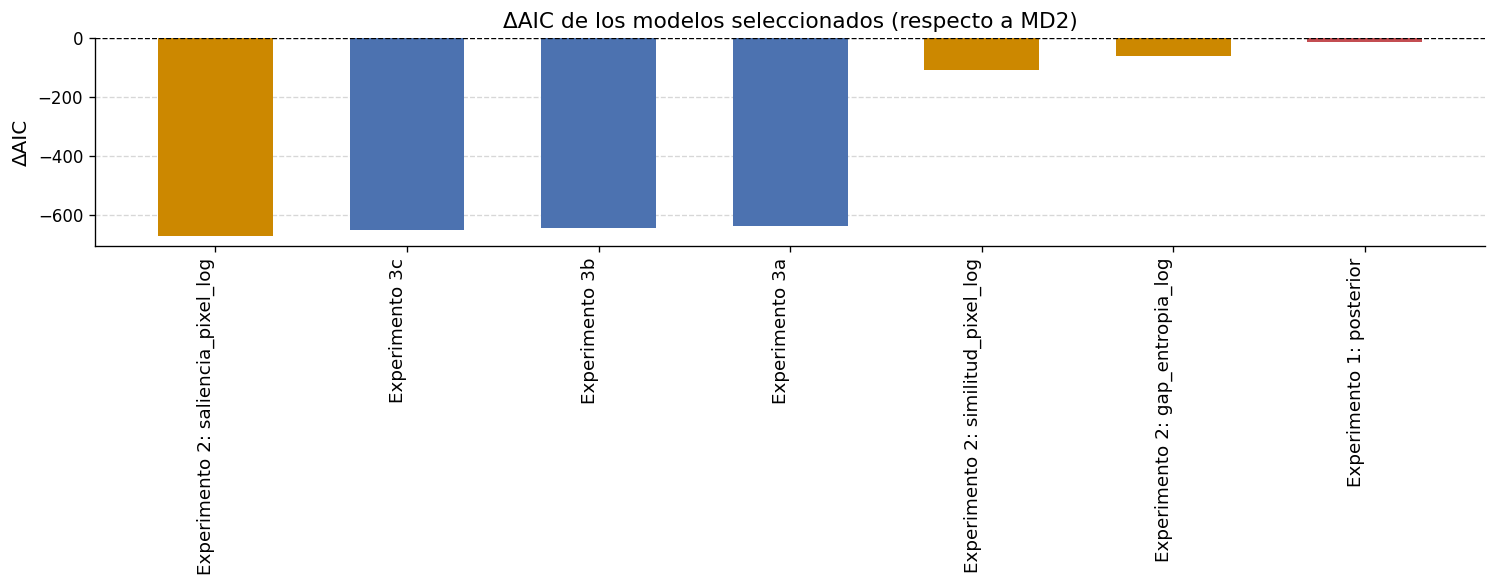
\includegraphics[width=0.85\textwidth]{chapters/05_resultados/images/AIC-final.png}
\caption{$\Delta$AIC respecto al modelo base MD2 para los modelos combinados
(Experimentos 3a y 3b, en azul) y para cada variable incorporada individualmente
(Experimentos 1 y 2, en rojo y naranja respectivamente).}
\label{fig:aic_combinados}
\end{figure}